\documentclass[letterpaper,9pt,twocolumn,twoside,]{pinp}

%% Some pieces required from the pandoc template
\providecommand{\tightlist}{%
  \setlength{\itemsep}{0pt}\setlength{\parskip}{0pt}}

% Use the lineno option to display guide line numbers if required.
% Note that the use of elements such as single-column equations
% may affect the guide line number alignment.

\usepackage[T1]{fontenc}
\usepackage[utf8]{inputenc}

% pinp change: the geometry package layout settings need to be set here, not in pinp.cls
\geometry{layoutsize={0.95588\paperwidth,0.98864\paperheight},%
  layouthoffset=0.02206\paperwidth, layoutvoffset=0.00568\paperheight}

\definecolor{pinpblue}{HTML}{185FAF}  % imagecolorpicker on blue for new R logo
\definecolor{pnasbluetext}{RGB}{101,0,0} %



\title{Body Fat Percentage Estimation}

\author[]{Tudor Liu, Samuel Tsui, Shirley Wang, William Wang}


\setcounter{secnumdepth}{0}

% Please give the surname of the lead author for the running footer
\leadauthor{}

% Keywords are not mandatory, but authors are strongly encouraged to provide them. If provided, please include two to five keywords, separated by the pipe symbol, e.g:
 

\begin{abstract}
In pursuit of an efficient method for estimating body fat percentage,
this study endeavors to explore a model utilizing various body
measurements. The research group seeks to establish a linear model that
can calculate body fat percentage through the incorporation of pertinent
body metrics.
\end{abstract}

\dates{This version was compiled on \today} 


% initially we use doi so keep for backwards compatibility
% new name is doi_footer


\begin{document}

% Optional adjustment to line up main text (after abstract) of first page with line numbers, when using both lineno and twocolumn options.
% You should only change this length when you've finalised the article contents.
\verticaladjustment{-2pt}

\maketitle
\thispagestyle{firststyle}
\ifthenelse{\boolean{shortarticle}}{\ifthenelse{\boolean{singlecolumn}}{\abscontentformatted}{\abscontent}}{}

% If your first paragraph (i.e. with the \dropcap) contains a list environment (quote, quotation, theorem, definition, enumerate, itemize...), the line after the list may have some extra indentation. If this is the case, add \parshape=0 to the end of the list environment.


\hypertarget{introduction}{%
\subsection{Introduction}\label{introduction}}

In this report, we delve into the vital subject of Body Fat Percentage
Estimation. Our investigative journey is anchored by data sourced from
the esteemed Brigham Young University's Human Performance Research
Center. The focus is on male body fat percentage - a parameter of
paramount importance in the realms of health and fitness.

\hypertarget{data-overview}{%
\subsection{Data Overview}\label{data-overview}}

Measuring body fat percentage accurately is difficult and often
expensive. Our dataset includes precise body fat measurements and other
accessible metrics for 250 cases across 16 categories. We've simplified
the data for clear insights into body fat percentage essentials.

\hypertarget{data-refinement}{%
\subsection{Data Refinement}\label{data-refinement}}

We refined our dataset by calculating body fat percentage from
underwater weighing, omitting duplicate density values. We resolved a
redundancy by keeping abdominal over wrist measurements and standardized
weight and height to kilograms and centimeters for analytical
consistency.

\begin{table}[h]

\begin{tabular}{|c|c|c|c|c|c|c|}
\hline
Waist & 33.54 & 32.68 & 34.61 & 34.02 & 39.37 & 37.17\\
\hline
Abdomen  & 85.20  & 83.00 & 87.90 & 86.40 & 100.00& 94.40\\
\hline
Abdomen/2.54  & 33.54 & 32.68 & 34.61 & 34.02 & 39.37 & 37.17\\
\hline

\end{tabular}
\caption{Redundancy between waist and abdomen}
\label{table:label_here}
\end{table}

\hypertarget{stepwise-variable-selection}{%
\subsection{Stepwise variable
selection}\label{stepwise-variable-selection}}

From the table, forward and backward search selected different
variables. Yet, their AIC are very close to each other. Therefore, we
decided to do 10-folds cross validation.

\begin{table}[!h]

\begin{tabular}{|c|c|c|c|c|}
\hline
\multicolumn{1}{|c|}{} & \multicolumn{2}{c|}{Forward model} & \multicolumn{2}{c|}{Backward model}\\

Predictors  & Estimates  & p & Estimates & p\\
\hline
(Intercept)  & -32.57 & <0.001 & 5.04 & 0.547 \\

Abdopmen  & 0.88 & <0.001 & 0.82 & 0.547 \\

Weight  & -0.24 & <0.001 &  & \\

Wrist  & -1.76 & <0.001 & -1.73 & 0.001 \\

Bicep  & 0.24 & 0.121 &  &  \\

Age  & 0.06 & 0.045 & 0.07 & 0.017 \\

Thigh  & 0.18 &0.1421 & 0.22 & 0.084 \\

Height  &  &  &-0.11 & 0.035 \\

Neck  &  &  &-0.45 & 0.039 \\

Hip  &  &  &-0.19 & 0.135 \\

Forearm &  &  &0.30 & 0.124 \\
\hline
\multicolumn{1}{|c|}{Observations} & \multicolumn{2}{c|}{250} & \multicolumn{2}{c|}{250}\\
\multicolumn{1}{|c|}{$R^2$/$R^2$ adjusted}
& \multicolumn{2}{c|}{0.742/0.736} & \multicolumn{2}{c|}{0.747/0.739}\\
\multicolumn{1}{|c|}{AIC} & \multicolumn{2}{c|}{1443.187} & \multicolumn{2}{c|}{1442.736}\\
\hline

\end{tabular}
\caption{Forward and backward search with AIC}
\label{table:label_here}
\end{table}

\hypertarget{boxplot-of-rmse-and-mae}{%
\subsection{Boxplot of rmse and mae}\label{boxplot-of-rmse-and-mae}}

The boxplots show the distribution of mean absolute error and root mean
square error in the forward and backward model. In both comparisons of
mae and rmse, both models give a similar distribution. Even when
comparing the mean value of both errors, two models give approximately
the same result.

\begin{figure}

{\centering 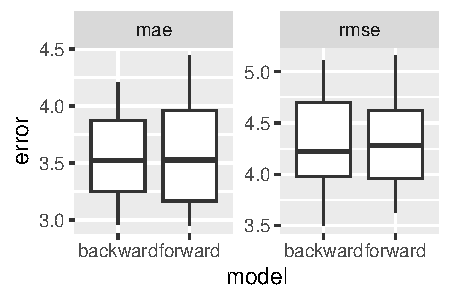
\includegraphics{Report_012E01_files/figure-latex/boxplot-1} 

}

\caption{Manual cross validation result}\label{fig:boxplot}
\end{figure}

\hypertarget{caret}{%
\subsection{Caret}\label{caret}}

Therefore, besides working the cross validation manually, we have done
it by using Caret as well.\\
From the caret method, the forward model seems to have smaller errors
than the backward model. Although Caret shows a slightly different
distribution of mae and rmse, there is still an uncertainty on which
model to choose.

\begin{figure}[!h]

{\centering 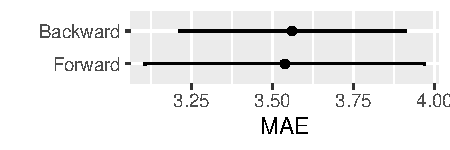
\includegraphics{Report_012E01_files/figure-latex/caret mae-1} 

}

\caption{Caret MAE figure}\label{fig:caret mae}
\end{figure}
\begin{figure}[!h]

{\centering 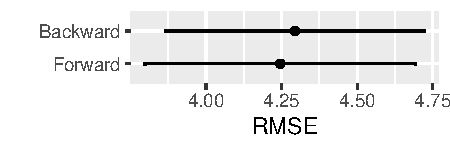
\includegraphics{Report_012E01_files/figure-latex/caret rmse-1} 

}

\caption{Caret RMSE figure}\label{fig:caret rmse}
\end{figure}
\begin{figure}[!h]

{\centering 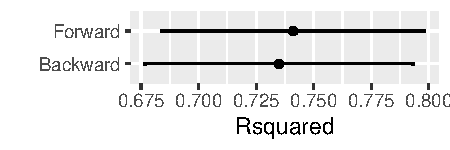
\includegraphics{Report_012E01_files/figure-latex/caret rsq-1} 

}

\caption{Caret Rsquared figure}\label{fig:caret rsq}
\end{figure}

\hypertarget{choose-forward-mode}{%
\subsection{Choose forward mode}\label{choose-forward-mode}}

The less the variables we need for the model, the easier people can get
their own percentage body fat. From table 2, forward model has selected
less attributes. To sum up, with the evidence in caret and considering
the amount of variables being used, we decided to use the forward model.

\hypertarget{assumption-checking}{%
\subsection{Assumption Checking}\label{assumption-checking}}

Before using the model to predict the average body fat percentage. It is
pivotal to ensure the model follows Linear regression assumptions.\\
\textbf{Independence}: the assumption states that all errors are
independent of each other. It is usually dealt within the experimental
design phase - before data collection , so it is not assessed in the
report.\\
\textbf{Normality:} the normality assumption assumes the errors follow
aa normal distribution. In figure 5, the residuals follow normal
distribution line, it suggests that the assumption of normality is
met.\\
\textbf{Linearity}: the assumption states relationship between fitted
values and percentage body fat are linear. Figure 6 shows a clear linear
relationship between body fat percentage and fitted value. Similar trend
is observed in figure 7, the residuals are roughly symmetric distributed
around the 0 axis , However, the model seems to overestimate percentage
body fat for fitted values above 30,it is trivial in this case as the
model is not designed to only predict body fat percentage for fitted
value above 30 and in overall ,only less than 10 percent of the data
lines in that interval. Therefore, the assumption is not violated.\\
\textbf{Homoscedasticity}: the assumption suggests the error variance
should remain constant across all levels of the independent variable,
Upon observing figure 3.3, the residuals are roughly evenly spread out
Except for residuals with a fitted value between 30 and 35 , suggesting
potential heteroscedasticity. However, since we have 250 observations
and only 9 of them lie in the fitted value interval between 30 and 35
,The heteroskedasticity is trivial as it affects a very narrow range of
the independent variable (between 30 and 35 less than 5\% of the
data).Thus, the model does not violate the assumption.

\begin{figure}[!h]

{\centering 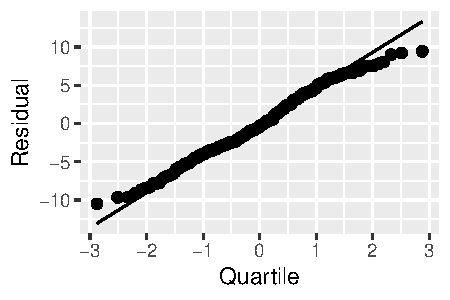
\includegraphics{Report_012E01_files/figure-latex/unnamed-chunk-1-1} 

}

\caption{qqplot of the residuals}\label{fig:unnamed-chunk-1}
\end{figure}

\begin{figure}[!h]

{\centering 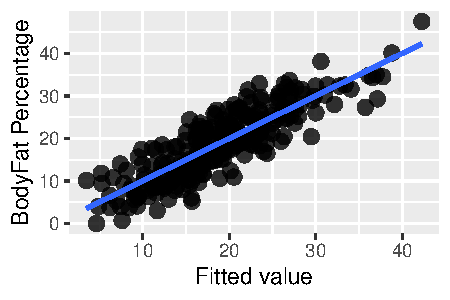
\includegraphics{Report_012E01_files/figure-latex/unnamed-chunk-2-1} 

}

\caption{relationship between bodyfate percentage and Fitted value}\label{fig:unnamed-chunk-2}
\end{figure}

\begin{figure}[!h]

{\centering 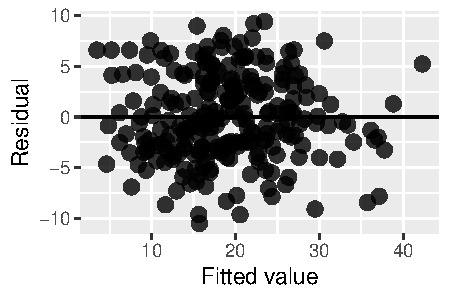
\includegraphics{Report_012E01_files/figure-latex/unnamed-chunk-3-1} 

}

\caption{relationship between residuals and Fitted value}\label{fig:unnamed-chunk-3}
\end{figure}

\hypertarget{result}{%
\subsection{Result}\label{result}}

As heath becomes a prevailing issue, the report is interested in
investigating the body fat percentage by predicting it indirectly
through related variables. The regression model for estimating Body fat
percentage is: Body fat percentage = -32.57 + 0.88 Abdomen -0.24 Weight
-1.76 Wrist + 0.24 Bicep + 0.06 Age + 0.18 Thigh According to the
regression found using Step-wise method, a percentage change in the
predictors results the coefficient percentage change in the body fat.

\hypertarget{discussion-and-conclusion}{%
\subsection{Discussion and Conclusion}\label{discussion-and-conclusion}}

One notable limitation of this study pertains to the sample size, which
may be considered inadequate for drawing comprehensive generalizations
or statistically robust conclusions. The relatively small sample size
(250 samples) utilized limits the extent to which the findings can be
extrapolated. A larger and more diverse sample size could be considered
to enhance the robustness for future researches, enabling a more
representative analysis of body composition factors.\\
For the utilization of Siri's equation, it is imperative to underscore
that Siri's equation operates based on a single variable (body density),
and the outcomes it provides are heavily contingent on the accuracy of
this singular metric. This equation may not fully account for the
complexities inherent in specific body composition characteristics.\\
Another noteworthy limitation of this study revolves around the
application of the AIC method. AIC operates under the assumption of
certain statistical conditions, such as model linearity, independence of
observations, and the absence of multicollinearity, among others.
Failure to fully satisfy these assumptions could potentially compromise
the accuracy and reliability of model selection, thus influencing the
interpretability of the results.\\
In summary, our linear regression model, with distinct coefficients,
shows promise for precise body fat estimation by considering variable
impacts. To maximize its potential, addressing limitations and further
refinement is crucial. This research contributes to evolving efficient
body composition assessment, with broad implications for health,
fitness, and science.

%\showmatmethods


\bibliography{pinp}
\bibliographystyle{jss}



\end{document}
